\subsection{\texorpdfstring{\(C^{r,s}\) 类流形（在 \(C^{r}\) 类流形之上）}{C\^{}\{r,s\} 类流形（在 C\^{}\{r\} 类流形之上）}}

在本节中，我们用 B 表示一个 \(C^{r}\) 类微分流形。

15.2.1. 设 X 是一个装备了映射 \(p: \mathbf{X} \to \mathbf{B}\) 的集合。我们称三元组 \(\theta = (\mathbf{V}, \psi, \mathbf{F})\) 为 X 在 B 上的卡，其中 V 是 X 的子集，F 是 K 上的 Banach 空间，\(\psi\) 是从 V 到 \(\mathbf{B} \times \mathbf{F}\) 的一个开子集上的双射，且满足 \(\mathrm{pr}_1 \circ \psi = p|\mathbf{V}\)。

设 \((\theta_{i})_{i\in I} = ((V_{i},\psi_{i},F_{i}))_{i\in I}\) 是 X 在 B 上的一个卡族。我们称诸 \(\theta_{i}\) 是 \(C^{r,s}\)-相容的，如果对 I 的每一对元素 \(i,j\)，下列两个条件都满足：

\begin{enumerate}
\def\labelenumi{\alph{enumi})}
\item
  \(\psi_i(V_i \cap V_j)\) 在 \(B \times F_i\) 中是开的，且 \(\psi_j(V_i \cap V_j)\) 在 \(B \times F_j\) 中是开的；
\item
  映射 \(\psi_i\circ\psi_j^{-1}\)（从 \(\psi_j(V_i\cap V_j)\) 到 \(\psi_i(V_i\cap V_j)\)）是一个 \(\mathrm{Id}_{\mathbf{B}}\)-态射，且是 \(\mathbf{C}^{r,s}\) 类的（15.1.7）。
\end{enumerate}

卡的一个族 \(((\mathrm{V}_i,\psi_i,\mathrm{F}_i))_{i\in I}\)（X 在 B 上的卡，它们 \(\mathbf{C}^{r,s}\)-相容且定义域 \(\mathrm{V}_i\) 覆盖 X）称为 X（在 B 上）的一个 \(\mathbf{C}^{r,s}\)-图册。两个 \(\mathbf{C}^{r,s}\)-图册称为等价的，如果它们的并仍是一个 \(\mathbf{C}^{r,s}\)-图册；\(\mathbf{C}^{r,s}\)-图册之间的等价关系是一个等价关系。\(\mathbf{C}^{r,s}\)-图册的一个等价类称为集合 X 上一个在 B 上的 \(\mathbf{C}^{r,s}\) 类流形结构；当希望指明 K 时，就写 \(\mathbf{C}_{\mathbb{K}}^{r,s}\) 以代替 \(\mathbf{C}^{r,s}\)。若 X 是 B 上的一个 \(\mathbf{C}^{r,s}\) 类流形，我们称 \(p\colon X\to B\) 为 X 的投影；若 \(\theta\) 是 X 在 B 上的一个卡，则我们称 \(\theta\) 是 \(\mathbf{C}^{r,s}\)-流形 X 的卡，如果 \(\theta\) 属于定义 X 结构的等价类中的某个图册。

设 X 是 B 上的一个 \(C^{r,s}\) 类流形，其投影为 p。则在 X 上存在

一个 \(\mathbf{C}^{r}\) 类微分流形结构，且是唯一的，使得对每个卡 \((V,\psi,F)\)（\(\mathbf{C}^{r,s}\)-流形 X 的卡），V 在 X 中是开的，且 \(\psi\) 是一个 \(\mathbf{C}^{r}\)-同构，它把 X 的开子流形 V 映到 \(\psi(V)\)（\(\mathbf{B}\times F\) 的开子流形）上。若给 X 装备这个结构，则映射 \(p:X\to B\) 是一个 \(\mathbf{C}^{r}\) 类的浸没。

设 \(b \in \mathbf{B}\)，并设 \(\mathbf{X}_b = p^{-1}(b)\)。存在一个 \(\mathbf{C}^s\) 类的 K-流形结构（\(\mathbf{X}_b\) 上的结构），且是唯一的，使得对每个卡 \(\theta = (\mathbf{V}, \psi, \mathbf{F})\)（\(\mathbf{C}^{r,s}\)-流形 \(\mathbf{X}\) 的卡），三元组 \(\theta_b = (\mathbf{V} \cap \mathbf{X}_b, \operatorname{pr}_2 \circ \psi | (\mathbf{V} \cap \mathbf{X}_b), \mathbf{F})\) 是流形 \(\mathbf{X}_b\) 的卡。这个结构之下的 \(\mathbf{C}^r\) 类微分流形结构是由上面定义的 \(\mathbf{C}^r\) 类微分流形结构（\(\mathbf{X}\) 上的结构）诱导的。
% semantic-fragments: legacy-input-seam
\relax{}
15.2.3. 例

\begin{enumerate}
\def\labelenumi{(\roman{enumi})}
\item
  当 B 退化为一点时，B 上的 \(C_{K}^{r,s}\) 类流形的概念等价于 \(C^{s}\) 类 K-流形的概念。
\item
  设 Z 是一个 \(C^{s}\) 类 K-流形；取 \(X = B \times Z\) 与 \(p = pr_{1}\)。在 X 上存在、且仅存在一个 B 上的 \(C^{r,s}\) 类流形结构，使得对 Z 的每个卡 \((U, \psi, L)\)，\((B \times U, Id_{B} \times \psi, L)\) 都是 \(C^{r,s}\) -流形 X 的一个卡。
\item
  设 X 是 B 上的一个 \(C^{r,s}\) 类流形，Y 是 X 的一个开子集。由 X 的结构诱导的 Y 的 \(C^{r,s}\) 类流形结构，其定义与流形情形中的做法相同（参见 5.2.3）。
\item
  设 M 是一个以 B 为底、\(C^{r}\) 类的 K 上的向量丛（7.3.4），\(\pi\) 是它到 B 上的投影。在 M 上存在、且仅存在一个 B 上的 \(C_{K}^{r,\omega}\) 类流形结构，使得若 \((\mathbf{U},\psi,\mathbf{F})\) 是 M 的一个 K-向量卡（8.8.1），则三元组 \((\pi^{-1}(\mathbf{U}),\psi,\mathbf{F})\) 是 \(C_{K}^{r,\omega}\) -流形 M 的一个卡。
\end{enumerate}

15.2.4. 设 X 是 B 上的一个 \(C^{r,s}\) 类流形，p 是其投影，L 是一个 K-Banach 空间，f 是 X 到 L 中的一个映射。我们说 f 是 \(C^{r,s}\) 类的，如果对流形 X 的每个卡 (V, \(\psi\) , F)（这里 X 视为 \(C^{r,s}\) -流形），映射 ( \(f|V) \circ \psi^{-1}\) （从 \(\psi(V)\) 到 L 中）是 \(C^{r,s}\) 类的（15.1.6）。这样的映射是 \(C^{r}\) 类的，并且它在 \(X_{b}\) （\(b \in B\)）上的限制是 \(C^{s}\) 类的。

15.2.5. 设 \(g: \mathbf{B} \to \mathbf{B}'\) 是 \(\mathbf{C}^{r}\) 类微分流形的一个态射，并设

\pandocbounded{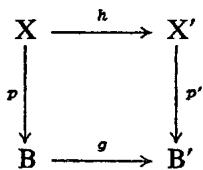
\includegraphics[keepaspectratio]{images/part001_9e08a31f.jpg}}

X（相应地，X'）是 B（相应地，B'）上的一个 \(C^{r,s}\) 类流形，h 是 X 到 X' 中的一个映射。我们说 h 是一个 \(C^{r,s}\) 类 g-态射，如果下列三个条件得到满足：

\begin{enumerate}
\def\labelenumi{\alph{enumi})}
\item
  \(p^{\prime}\circ h = g\circ p;\)
\item
  h 连续；
\item
  对每个卡 \((\mathrm{V}^{\prime},\psi^{\prime},\mathrm{F}^{\prime})\) （\(C^{r,s}\) -流形 \(X^{\prime}\) 的卡），映射 \(pr_{2}\circ\psi^{\prime}\circ h\) 从 \(V=h^{-1}(V^{\prime})\) 到 \(F^{\prime}\) 是
\end{enumerate}

\(\mathbf{C}^{r,s}\) 类的（按 15.2.4 的意义），这里开集 V 赋有由 X 诱导的结构（15.2.3, (iii)）。

当 \(\mathbf{B} = \mathbf{B}'\) 且 \(g = \mathrm{Id}_{\mathbf{B}}\) 时，我们也称 \(h\) 为一个 \(\mathbf{C}^{r,s}\) 类 B-态射。

为使一个 \(C^{r,s}\) 类 B-态射是一个 \(C^{r,s}\) 类 B-同构，只需它是一个 \(C^{1}\) 类同构。

设 \(g': B' \to B''\) 是 \(C^r\) 类流形的一个态射，并设 \(X''\) 是一个 \(C^{r,s}\) 类流形，其底为 \(B''\) 。若 \(h: X \to X'\) 是一个 \(g\) -态射且为 \(C^{r,s}\) 类，而 \(h': X' \to X''\) 是一个 \(g'\) -态射且为 \(C^{r,s}\) 类，则 \(h' \circ h\) 是一个 \((g' \circ g)\) -态射且为 \(C^{r,s}\) 类。

15.2.6. 设 X 是 B 上的一个 \(\mathbf{C}_{\mathbf{R}}^{r,s}\) 类流形，\(p\) 是其投影；我们假设 \(s \neq \omega\) ，X 是分离的，且 \(p\) 是逆紧的（TG, I, § 10, no. 1）。于是，对每个 \(b \in \mathbf{B}\) ，存在 \(b\) 的一个开邻域 U 以及一个 \(\mathbf{C}^{r,s}\) -同构（从 \(p^{-1}(\mathbf{U})\) 到 \(\mathbf{U} \times \mathbf{X}_b\) 上），其中 \(\mathbf{X}_b = p^{-1}(b)\) 。

15.2.7. 设 X 是 B 上的一个 \(C_{K}^{r,s}\) 类流形，p 是其投影，\(\sigma: B \to X\) 是一个 \(C^{r}\) 类截面。我们称一个 \(C_{K}^{r,s}\) 类管状邻域（\(\sigma\) 的）为如下的三元组 (M, N, \(\varphi\) )：其中 M 是一个以 B 为底、\(C^{r}\) 类的 K-向量丛，N 是 \(\sigma(\mathbf{B})\) 在 X 中的一个开邻域，而 \(\varphi\) 是一个 \(C_{K}^{r,s}\) 类 B-同构（从 N 到 M 的一个开子集上，参见 15.2.3 (iv)），它把截面 \(\sigma\) 映为 M 的零截面。

假设 \(s \geqslant r + 1\) ，并且流形 B 是仿紧的、具有 \(\mathbf{C}^{r}\) 类单位分解（5.3.6）；则存在 \(\mathbf{C}_{\mathbb{K}}^{r,s}\) 类管状邻域（\(\sigma\) 的）。

